\chapter{Graphite}
\begin{figure}[!htp]
	\centering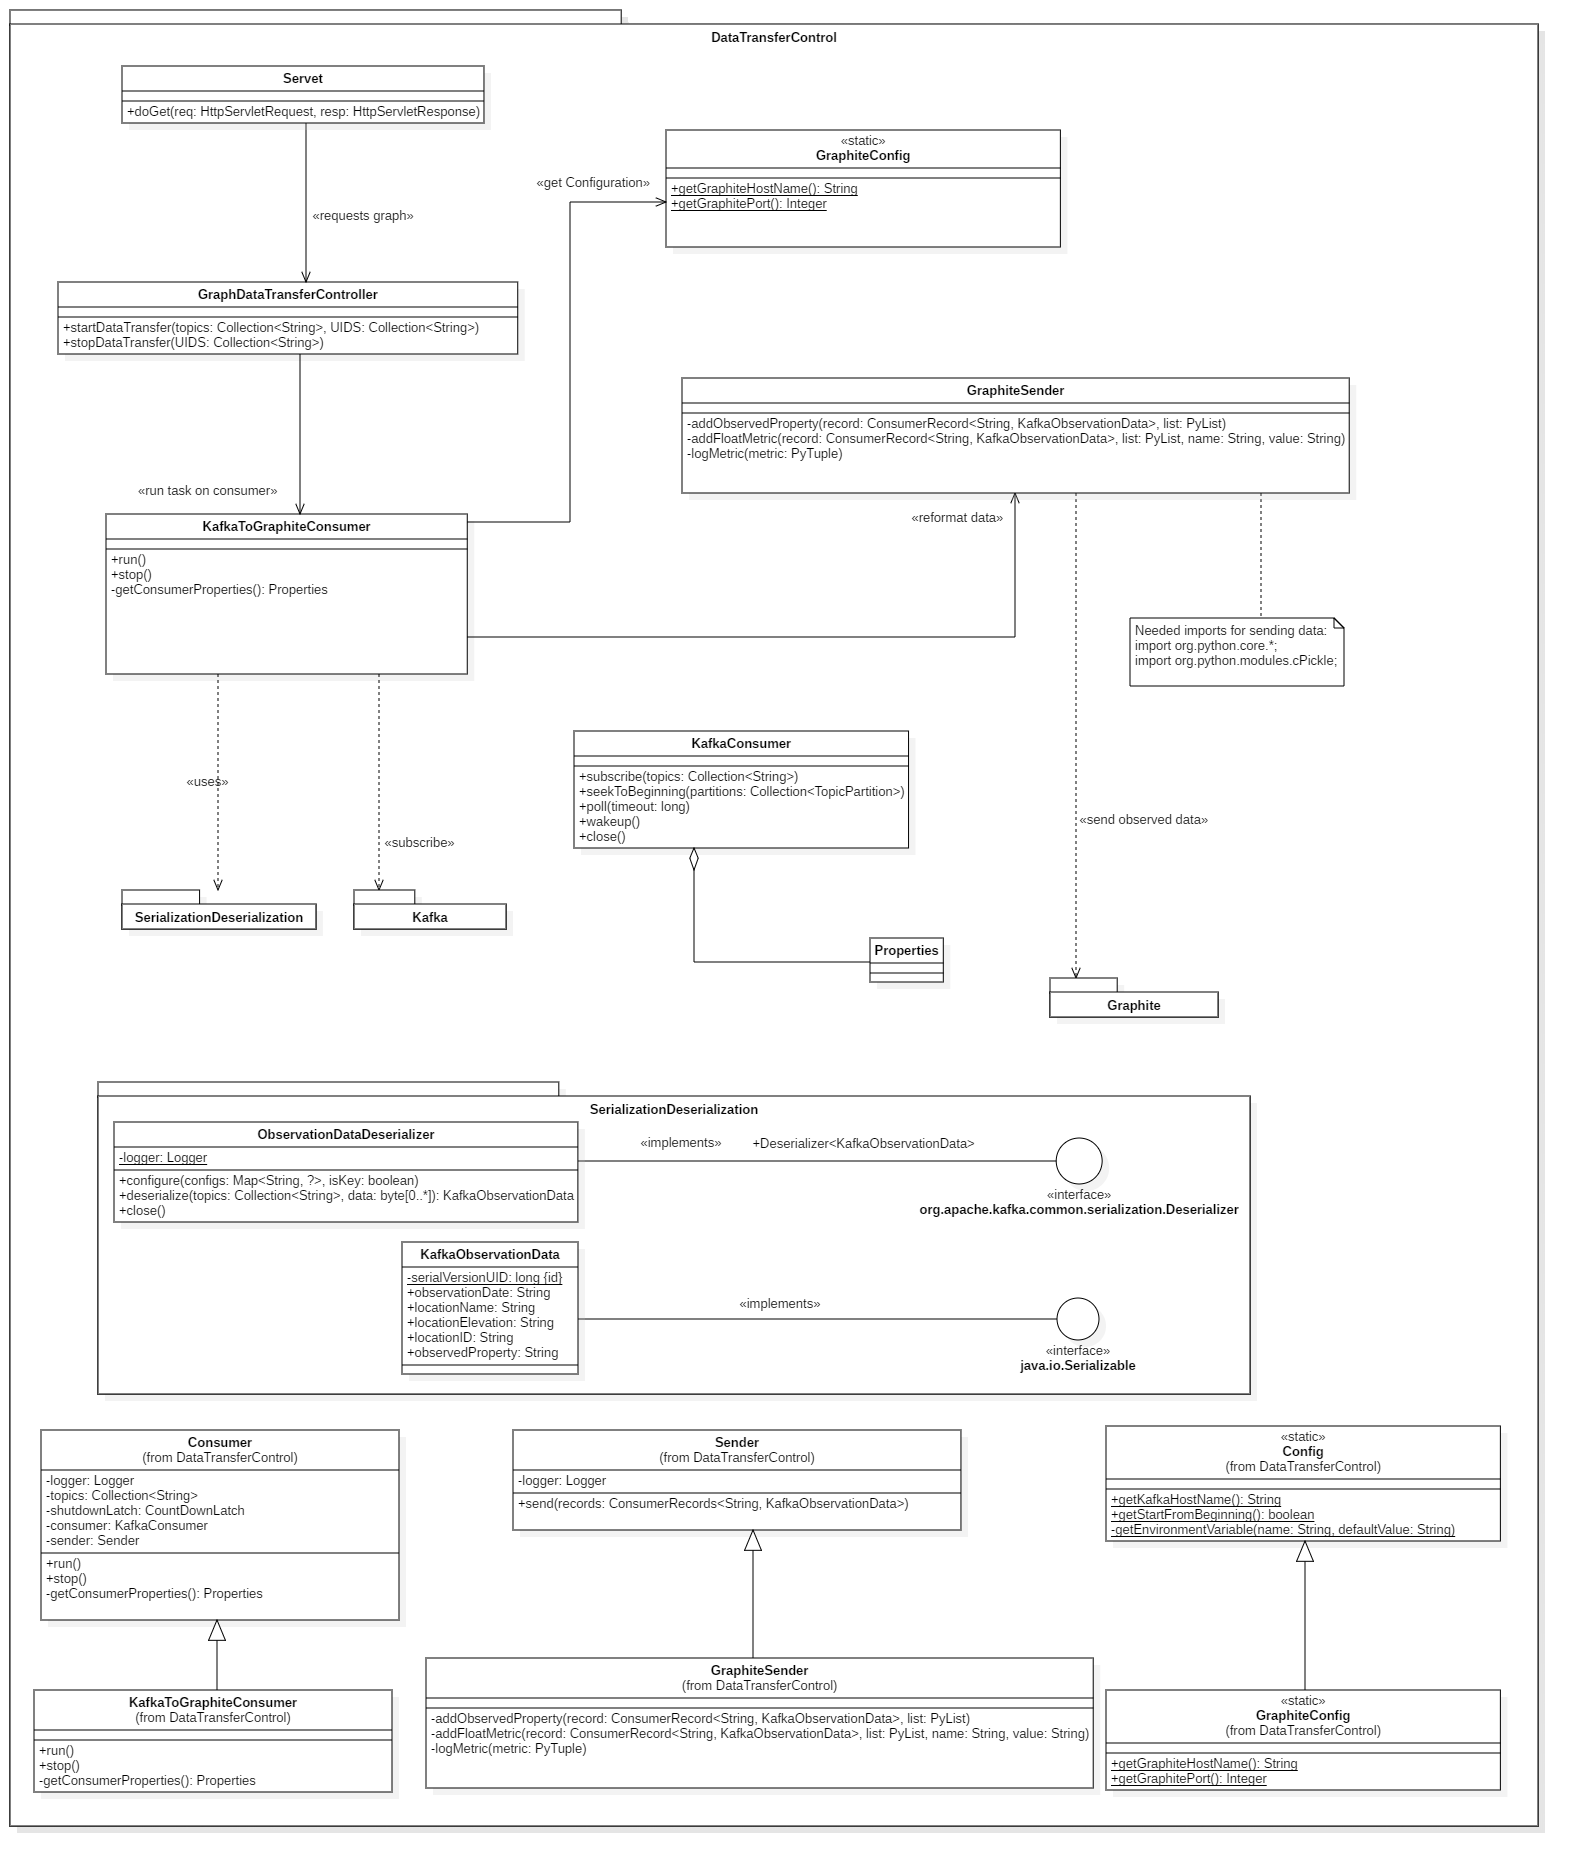
\includegraphics[width=\linewidth]{images/graphite/graphiteClassDiagram}
	\caption{Klassendiagramm Graphite}
\end{figure}
\section{Package DataTransferControl}{
\label{DataTransferControl}\hypertarget{DataTransferControl}{}
\hskip -.05in
\hbox to \hsize{\textit{ Package Contents\hfil Page}}
\vskip .13in
\hbox{{\bf  Classes}}
\entityintro{Collection}{DataTransferControl.Collection}{A Collection that stores multiple objects of one type}
\entityintro{Config}{DataTransferControl.Config}{The specified configuration-object that stores all needed configurations for the connection from Kafka to another specified component}
\entityintro{Consumer}{DataTransferControl.Consumer}{Consumes data from Kafka}
\entityintro{ConsumerRecord}{DataTransferControl.ConsumerRecord}{One single record of data from Kafka}
\entityintro{ConsumerRecords}{DataTransferControl.ConsumerRecords}{Multiple records of data from Kafka}
\entityintro{GraphDataTransferController}{DataTransferControl.GraphDataTransferController}{The Control-Unit in charge of creating and destroying KafkaToGraphiteConsumer as well as passing on the users request.}
\entityintro{GraphiteConfig}{DataTransferControl.GraphiteConfig}{The specified configuration-object that stores all needed configurations for the connection from Kafka to Graphite}
\entityintro{GraphiteSender}{DataTransferControl.GraphiteSender}{Reformats the data and sends it to Graphite}
\entityintro{KafkaConsumer}{DataTransferControl.KafkaConsumer}{The Kafka Consumer is described in Apache-Kafka and will only be included in this diagram for a better understanding of the required functionality.}
\entityintro{KafkaToGraphiteConsumer}{DataTransferControl.KafkaToGraphiteConsumer}{Receives the data from Kafka and sends it to Graphite}
\entityintro{Properties}{DataTransferControl.Properties}{The Properties of the KafkaConsumer, using Java.Util.Properties}
\entityintro{Sender}{DataTransferControl.Sender}{Reformats the data and sends it to another component}
\entityintro{Servet}{DataTransferControl.Servet}{A Servlet, which accepts the user-requests from the webinterface and passes them on to the responsible structures}
\vskip .1in
\vskip .1in
\subsection{\label{DataTransferControl.Collection}Class Collection}{
\hypertarget{DataTransferControl.Collection}{}\vskip .1in 
A Collection that stores multiple objects of one type\vskip .1in 
\subsubsection{Declaration}{
\begin{lstlisting}[frame=none]
public class Collection
 extends java.lang.Object\end{lstlisting}
\subsubsection{Constructor summary}{
\begin{verse}
\hyperlink{DataTransferControl.Collection()}{{\bf Collection()}} Default constructor\\
\end{verse}
}
\subsubsection{Constructors}{
\vskip -2em
\begin{itemize}
\item{ 
\index{Collection()}
\hypertarget{DataTransferControl.Collection()}{{\bf  Collection}\\}
\begin{lstlisting}[frame=none]
public Collection()\end{lstlisting} %end signature
\begin{itemize}
\item{
{\bf  Description}

Default constructor
}
\end{itemize}
}%end item
\end{itemize}
}
}
\subsection{\label{DataTransferControl.Config}Class Config}{
\hypertarget{DataTransferControl.Config}{}\vskip .1in 
The specified configuration-object that stores all needed configurations for the connection from Kafka to another specified component\vskip .1in 
\begin{figure}[!htp]
	\centering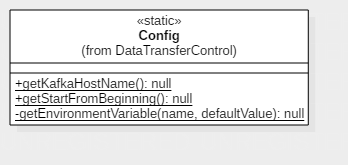
\includegraphics[width=0.4\linewidth]{images/graphite/classes/ClassConfig}
\end{figure} 
\subsubsection{Declaration}{
\begin{lstlisting}[frame=none]
public class Config
 extends java.lang.Object\end{lstlisting}
\subsubsection{All known subclasses}{GraphiteConfig\small{\refdefined{DataTransferControl.GraphiteConfig}}}
\subsubsection{Constructor summary}{
\begin{verse}
\hyperlink{DataTransferControl.Config()}{{\bf Config()}} Default constructor\\
\end{verse}
}
\subsubsection{Method summary}{
\begin{verse}
\hyperlink{DataTransferControl.Config.getKafkaHostName()}{{\bf getKafkaHostName()}} Gets the Kafka-host-name\\
\hyperlink{DataTransferControl.Config.getStartFromBeginning()}{{\bf getStartFromBeginning()}} Returns whether a start from the beginning is required\\
\end{verse}
}
\subsubsection{Constructors}{
\vskip -2em
\begin{itemize}
\item{ 
\index{Config()}
\hypertarget{DataTransferControl.Config()}{{\bf  Config}\\}
\begin{lstlisting}[frame=none]
public Config()\end{lstlisting} %end signature
\begin{itemize}
\item{
{\bf  Description}

Default constructor
}
\end{itemize}
}%end item
\end{itemize}
}
\subsubsection{Methods}{
\vskip -2em
\begin{itemize}
\item{ 
\index{getKafkaHostName()}
\hypertarget{DataTransferControl.Config.getKafkaHostName()}{{\bf  getKafkaHostName}\\}
\begin{lstlisting}[frame=none]
public static java.lang.String getKafkaHostName()\end{lstlisting} %end signature
\begin{itemize}
\item{
{\bf  Description}

Gets the Kafka-host-name
}
\item{{\bf  Returns} -- 
The host-name of Kafka 
}%end item
\end{itemize}
}%end item
\item{ 
\index{getStartFromBeginning()}
\hypertarget{DataTransferControl.Config.getStartFromBeginning()}{{\bf  getStartFromBeginning}\\}
\begin{lstlisting}[frame=none]
public static boolean getStartFromBeginning()\end{lstlisting} %end signature
\begin{itemize}
\item{
{\bf  Description}

Returns whether a start from the beginning is required
}
\item{{\bf  Returns} -- 
Tells us whether a start from the beginning is required 
}%end item
\end{itemize}
}%end item
\end{itemize}
}
}
\subsection{\label{DataTransferControl.Consumer}Class Consumer}{
\hypertarget{DataTransferControl.Consumer}{}\vskip .1in 
Consumes data from Kafka\vskip .1in 
\begin{figure}[!htp]
	\centering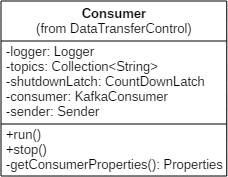
\includegraphics[width=0.3\linewidth]{images/graphite/classes/ClassConsumer}
\end{figure} 
\subsubsection{Declaration}{
\begin{lstlisting}[frame=none]
public class Consumer
 extends java.lang.Object\end{lstlisting}
\subsubsection{All known subclasses}{KafkaToGraphiteConsumer\small{\refdefined{DataTransferControl.KafkaToGraphiteConsumer}}}
\subsubsection{Constructor summary}{
\begin{verse}
\hyperlink{DataTransferControl.Consumer()}{{\bf Consumer()}} Default constructor\\
\end{verse}
}
\subsubsection{Method summary}{
\begin{verse}
\hyperlink{DataTransferControl.Consumer.run()}{{\bf run()}} Starts the transferring-process\\
\hyperlink{DataTransferControl.Consumer.stop()}{{\bf stop()}} Stops the transferring-process\\
\end{verse}
}
\subsubsection{Constructors}{
\vskip -2em
\begin{itemize}
\item{ 
\index{Consumer()}
\hypertarget{DataTransferControl.Consumer()}{{\bf  Consumer}\\}
\begin{lstlisting}[frame=none]
public Consumer()\end{lstlisting} %end signature
\begin{itemize}
\item{
{\bf  Description}

Default constructor
}
\end{itemize}
}%end item
\end{itemize}
}
\subsubsection{Methods}{
\vskip -2em
\begin{itemize}
\item{ 
\index{run()}
\hypertarget{DataTransferControl.Consumer.run()}{{\bf  run}\\}
\begin{lstlisting}[frame=none]
public void run()\end{lstlisting} %end signature
\begin{itemize}
\item{
{\bf  Description}

Starts the transferring-process
}
\end{itemize}
}%end item
\item{ 
\index{stop()}
\hypertarget{DataTransferControl.Consumer.stop()}{{\bf  stop}\\}
\begin{lstlisting}[frame=none]
public void stop()\end{lstlisting} %end signature
\begin{itemize}
\item{
{\bf  Description}

Stops the transferring-process
}
\end{itemize}
}%end item
\end{itemize}
}
}
\subsection{\label{DataTransferControl.ConsumerRecord}Class ConsumerRecord}{
\hypertarget{DataTransferControl.ConsumerRecord}{}\vskip .1in 
One single record of data from Kafka\vskip .1in 
\begin{figure}[!htp]
	\centering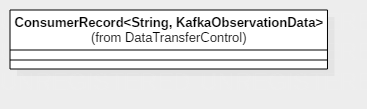
\includegraphics[width=0.2\linewidth]{images/graphite/classes/ClassConsumerRecord}
\end{figure} 
\subsubsection{Declaration}{
\begin{lstlisting}[frame=none]
public class ConsumerRecord
 extends java.lang.Object\end{lstlisting}
\subsubsection{Constructor summary}{
\begin{verse}
\hyperlink{DataTransferControl.ConsumerRecord()}{{\bf ConsumerRecord()}} Default constructor\\
\end{verse}
}
\subsubsection{Constructors}{
\vskip -2em
\begin{itemize}
\item{ 
\index{ConsumerRecord()}
\hypertarget{DataTransferControl.ConsumerRecord()}{{\bf  ConsumerRecord}\\}
\begin{lstlisting}[frame=none]
public ConsumerRecord()\end{lstlisting} %end signature
\begin{itemize}
\item{
{\bf  Description}

Default constructor
}
\end{itemize}
}%end item
\end{itemize}
}
}
\subsection{\label{DataTransferControl.ConsumerRecords}Class ConsumerRecords}{
\hypertarget{DataTransferControl.ConsumerRecords}{}\vskip .1in 
Multiple records of data from Kafka\vskip .1in 
\begin{figure}[!htp]
	\centering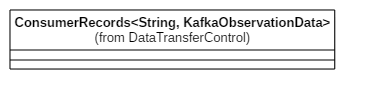
\includegraphics[width=0.2\linewidth]{images/graphite/classes/ClassConsumerRecords}
\end{figure} 
\subsubsection{Declaration}{
\begin{lstlisting}[frame=none]
public class ConsumerRecords
 extends java.lang.Object\end{lstlisting}
\subsubsection{Constructor summary}{
\begin{verse}
\hyperlink{DataTransferControl.ConsumerRecords()}{{\bf ConsumerRecords()}} Default constructor\\
\end{verse}
}
\subsubsection{Constructors}{
\vskip -2em
\begin{itemize}
\item{ 
\index{ConsumerRecords()}
\hypertarget{DataTransferControl.ConsumerRecords()}{{\bf  ConsumerRecords}\\}
\begin{lstlisting}[frame=none]
public ConsumerRecords()\end{lstlisting} %end signature
\begin{itemize}
\item{
{\bf  Description}

Default constructor
}
\end{itemize}
}%end item
\end{itemize}
}
}
\subsection{\label{DataTransferControl.GraphDataTransferController}Class GraphDataTransferController}{
\hypertarget{DataTransferControl.GraphDataTransferController}{}\vskip .1in 
The Control-Unit in charge of creating and destroying KafkaToGraphiteConsumer as well as passing on the users request.\vskip .1in 
\begin{figure}[!htp]
	\centering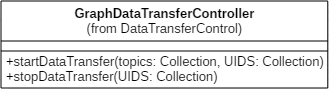
\includegraphics[width=0.6\linewidth]{images/graphite/classes/ClassGraphDataTransferController}
\end{figure} 
\subsubsection{Declaration}{
\begin{lstlisting}[frame=none]
public class GraphDataTransferController
 extends java.lang.Object\end{lstlisting}
\subsubsection{Constructor summary}{
\begin{verse}
\hyperlink{DataTransferControl.GraphDataTransferController()}{{\bf GraphDataTransferController()}} Default constructor\\
\end{verse}
}
\subsubsection{Method summary}{
\begin{verse}
\hyperlink{DataTransferControl.GraphDataTransferController.startDataTransfer(<any>, <any>)}{{\bf startDataTransfer(, )}} Starts data-transfer\\
\hyperlink{DataTransferControl.GraphDataTransferController.stopDataTransfer(<any>)}{{\bf stopDataTransfer()}} Stoppt den Datentransfer.\\
\end{verse}
}
\subsubsection{Constructors}{
\vskip -2em
\begin{itemize}
\item{ 
\index{GraphDataTransferController()}
\hypertarget{DataTransferControl.GraphDataTransferController()}{{\bf  GraphDataTransferController}\\}
\begin{lstlisting}[frame=none]
public GraphDataTransferController()\end{lstlisting} %end signature
\begin{itemize}
\item{
{\bf  Description}

Default constructor
}
\end{itemize}
}%end item
\end{itemize}
}
\subsubsection{Methods}{
\vskip -2em
\begin{itemize}
\item{ 
\index{startDataTransfer(, )}
\hypertarget{DataTransferControl.GraphDataTransferController.startDataTransfer(<any>, <any>)}{{\bf  startDataTransfer}\\}
\begin{lstlisting}[frame=none]
public void startDataTransfer(Collection<String> topics,Collection<String> UIDS)\end{lstlisting} %end signature
\begin{itemize}
\item{
{\bf  Description}

Starts data-transfer
}
\item{
{\bf  Parameters}
  \begin{itemize}
   \item{
\texttt{topics} -- Kafka-Topics that should be subscribed}
   \item{
\texttt{UIDS} -- The unique identifiers, that tell us which data should be transfered. Everything else will be ignored.}
  \end{itemize}
}%end item
\end{itemize}
}%end item
\item{ 
\index{stopDataTransfer()}
\hypertarget{DataTransferControl.GraphDataTransferController.stopDataTransfer(<any>)}{{\bf  stopDataTransfer}\\}
\begin{lstlisting}[frame=none]
public void stopDataTransfer(Collection<String> UIDS)\end{lstlisting} %end signature
\begin{itemize}
\item{
{\bf  Description}

Stoppt den Datentransfer.
}
\item{
{\bf  Parameters}
  \begin{itemize}
   \item{
\texttt{UIDS} -- The unique identifiers, that tell us which data should no longer be transfered. Everything else will be ignored.}
  \end{itemize}
}%end item
\end{itemize}
}%end item
\end{itemize}
}
}
\subsection{\label{DataTransferControl.GraphiteConfig}Class GraphiteConfig}{
\hypertarget{DataTransferControl.GraphiteConfig}{}\vskip .1in 
The specified configuration-object that stores all needed configurations for the connection from Kafka to Graphite\vskip .1in 
\begin{figure}[!htp]
	\centering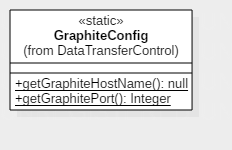
\includegraphics[width=0.25\linewidth]{images/graphite/classes/ClassGraphiteConfig}
\end{figure} 
\subsubsection{Declaration}{
\begin{lstlisting}[frame=none]
public class GraphiteConfig
 extends DataTransferControl.Config\end{lstlisting}
\subsubsection{Constructor summary}{
\begin{verse}
\hyperlink{DataTransferControl.GraphiteConfig()}{{\bf GraphiteConfig()}} Default constructor\\
\end{verse}
}
\subsubsection{Method summary}{
\begin{verse}
\hyperlink{DataTransferControl.GraphiteConfig.getGraphiteHostName()}{{\bf getGraphiteHostName()}} Returns the host-name of Graphite\\
\hyperlink{DataTransferControl.GraphiteConfig.getGraphitePort()}{{\bf getGraphitePort()}} Returns the port of the Graphite-connection\\
\end{verse}
}
\subsubsection{Constructors}{
\vskip -2em
\begin{itemize}
\item{ 
\index{GraphiteConfig()}
\hypertarget{DataTransferControl.GraphiteConfig()}{{\bf  GraphiteConfig}\\}
\begin{lstlisting}[frame=none]
public GraphiteConfig()\end{lstlisting} %end signature
\begin{itemize}
\item{
{\bf  Description}

Default constructor
}
\end{itemize}
}%end item
\end{itemize}
}
\subsubsection{Methods}{
\vskip -2em
\begin{itemize}
\item{ 
\index{getGraphiteHostName()}
\hypertarget{DataTransferControl.GraphiteConfig.getGraphiteHostName()}{{\bf  getGraphiteHostName}\\}
\begin{lstlisting}[frame=none]
public static java.lang.String getGraphiteHostName()\end{lstlisting} %end signature
\begin{itemize}
\item{
{\bf  Description}

Returns the host-name of Graphite
}
\item{{\bf  Returns} -- 
The Graphite-host-name 
}%end item
\end{itemize}
}%end item
\item{ 
\index{getGraphitePort()}
\hypertarget{DataTransferControl.GraphiteConfig.getGraphitePort()}{{\bf  getGraphitePort}\\}
\begin{lstlisting}[frame=none]
public static java.lang.Integer getGraphitePort()\end{lstlisting} %end signature
\begin{itemize}
\item{
{\bf  Description}

Returns the port of the Graphite-connection
}
\item{{\bf  Returns} -- 
The port of the Graphite-connection 
}%end item
\end{itemize}
}%end item
\end{itemize}
}
\subsubsection{Members inherited from class Config }{
\texttt{DataTransferControl.Config} {\small 
\refdefined{DataTransferControl.Config}}
{\small 

\vskip -2em
\begin{itemize}
\item{\vskip -1.5ex 
\texttt{public static String {\bf  getKafkaHostName}()
}%end signature
}%end item
\item{\vskip -1.5ex 
\texttt{public static boolean {\bf  getStartFromBeginning}()
}%end signature
}%end item
\end{itemize}
}
}
\subsection{\label{DataTransferControl.GraphiteSender}Class GraphiteSender}{
\hypertarget{DataTransferControl.GraphiteSender}{}\vskip .1in 
Reformats the data and sends it to Graphite\vskip .1in 
\begin{figure}[!htp]
	\centering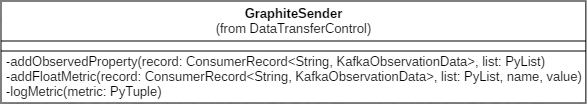
\includegraphics[width=0.8\linewidth]{images/graphite/classes/ClassGraphiteSender}
\end{figure} 
\subsubsection{Declaration}{
\begin{lstlisting}[frame=none]
public class GraphiteSender
 extends DataTransferControl.Sender\end{lstlisting}
\subsubsection{Constructor summary}{
\begin{verse}
\hyperlink{DataTransferControl.GraphiteSender()}{{\bf GraphiteSender()}} Default constructor\\
\end{verse}
}
\subsubsection{Constructors}{
\vskip -2em
\begin{itemize}
\item{ 
\index{GraphiteSender()}
\hypertarget{DataTransferControl.GraphiteSender()}{{\bf  GraphiteSender}\\}
\begin{lstlisting}[frame=none]
public GraphiteSender()\end{lstlisting} %end signature
\begin{itemize}
\item{
{\bf  Description}

Default constructor
}
\end{itemize}
}%end item
\end{itemize}
}
\subsubsection{Members inherited from class Sender }{
\texttt{DataTransferControl.Sender} {\small 
\refdefined{DataTransferControl.Sender}}
{\small 

\vskip -2em
\begin{itemize}
\item{\vskip -1.5ex 
\texttt{public void {\bf  send}(\texttt{} {\bf  records})
}%end signature
}%end item
\end{itemize}
}
}
\subsection{\label{DataTransferControl.KafkaConsumer}Class KafkaConsumer}{
\hypertarget{DataTransferControl.KafkaConsumer}{}\vskip .1in 
The Kafka Consumer is described in Apache-Kafka and will only be included in this diagram for a better understanding of the required functionality.\vskip .1in 
\begin{figure}[!htp]
	\centering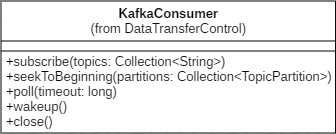
\includegraphics[width=0.4\linewidth]{images/graphite/classes/ClassKafkaConsumer}
\end{figure} 
\subsubsection{Declaration}{
\begin{lstlisting}[frame=none]
public class KafkaConsumer
 extends java.lang.Object\end{lstlisting}
\subsubsection{Constructor summary}{
\begin{verse}
\hyperlink{DataTransferControl.KafkaConsumer()}{{\bf KafkaConsumer()}} Default constructor\\
\end{verse}
}
\subsubsection{Method summary}{
\begin{verse}
\hyperlink{DataTransferControl.KafkaConsumer.close()}{{\bf close()}} Closes the KafkaConsumer\\
\hyperlink{DataTransferControl.KafkaConsumer.poll(long)}{{\bf poll(long)}} Gathers the data\\
\hyperlink{DataTransferControl.KafkaConsumer.seekToBeginning(<any>)}{{\bf seekToBeginning()}} Jumps to the beginning of an existing record\\
\hyperlink{DataTransferControl.KafkaConsumer.subscribe(<any>)}{{\bf subscribe()}} The Consumer subscribes Kafka-Topics.\\
\hyperlink{DataTransferControl.KafkaConsumer.wakeup()}{{\bf wakeup()}} Wakes up the KafkaConsumer, which then stops any current requests.\\
\end{verse}
}
\subsubsection{Constructors}{
\vskip -2em
\begin{itemize}
\item{ 
\index{KafkaConsumer()}
\hypertarget{DataTransferControl.KafkaConsumer()}{{\bf  KafkaConsumer}\\}
\begin{lstlisting}[frame=none]
public KafkaConsumer()\end{lstlisting} %end signature
\begin{itemize}
\item{
{\bf  Description}

Default constructor
}
\end{itemize}
}%end item
\end{itemize}
}
\subsubsection{Methods}{
\vskip -2em
\begin{itemize}
\item{ 
\index{close()}
\hypertarget{DataTransferControl.KafkaConsumer.close()}{{\bf  close}\\}
\begin{lstlisting}[frame=none]
public void close()\end{lstlisting} %end signature
\begin{itemize}
\item{
{\bf  Description}

Closes the KafkaConsumer
}
\end{itemize}
}%end item
\item{ 
\index{poll(long)}
\hypertarget{DataTransferControl.KafkaConsumer.poll(long)}{{\bf  poll}\\}
\begin{lstlisting}[frame=none]
public void poll(long timeout)\end{lstlisting} %end signature
\begin{itemize}
\item{
{\bf  Description}

Gathers the data
}
\item{
{\bf  Parameters}
  \begin{itemize}
   \item{
\texttt{timeout} -- A timeframe, limiting the longest possible duration of the poll request}
  \end{itemize}
}%end item
\end{itemize}
}%end item
\item{ 
\index{seekToBeginning()}
\hypertarget{DataTransferControl.KafkaConsumer.seekToBeginning(<any>)}{{\bf  seekToBeginning}\\}
\begin{lstlisting}[frame=none]
public void seekToBeginning(Collection<TopicPartition> partitions)\end{lstlisting} %end signature
\begin{itemize}
\item{
{\bf  Description}

Jumps to the beginning of an existing record
}
\item{
{\bf  Parameters}
  \begin{itemize}
   \item{
\texttt{partitions} -- Kafka-Partitions}
  \end{itemize}
}%end item
\end{itemize}
}%end item
\item{ 
\index{subscribe()}
\hypertarget{DataTransferControl.KafkaConsumer.subscribe(<any>)}{{\bf  subscribe}\\}
\begin{lstlisting}[frame=none]
public void subscribe(Collection<String> topics)\end{lstlisting} %end signature
\begin{itemize}
\item{
{\bf  Description}

The Consumer subscribes Kafka-Topics.
}
\item{
{\bf  Parameters}
  \begin{itemize}
   \item{
\texttt{topics} -- Kafka-Topics that should be subscribed}
  \end{itemize}
}%end item
\end{itemize}
}%end item
\item{ 
\index{wakeup()}
\hypertarget{DataTransferControl.KafkaConsumer.wakeup()}{{\bf  wakeup}\\}
\begin{lstlisting}[frame=none]
public void wakeup()\end{lstlisting} %end signature
\begin{itemize}
\item{
{\bf  Description}

Wakes up the KafkaConsumer, which then stops any current requests. Useful to limit polls in general.
}
\end{itemize}
}%end item
\end{itemize}
}
}
\subsection{\label{DataTransferControl.KafkaToGraphiteConsumer}Class KafkaToGraphiteConsumer}{
\hypertarget{DataTransferControl.KafkaToGraphiteConsumer}{}\vskip .1in 
Receives the data from Kafka and sends it to Graphite\vskip .1in 
\begin{figure}[!htp]
	\centering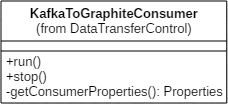
\includegraphics[width=0.3\linewidth]{images/graphite/classes/ClassKafkaToGraphiteConsumer}
\end{figure} 
\subsubsection{Declaration}{
\begin{lstlisting}[frame=none]
public class KafkaToGraphiteConsumer
 extends DataTransferControl.Consumer\end{lstlisting}
\subsubsection{Constructor summary}{
\begin{verse}
\hyperlink{DataTransferControl.KafkaToGraphiteConsumer()}{{\bf KafkaToGraphiteConsumer()}} Default constructor\\
\end{verse}
}
\subsubsection{Method summary}{
\begin{verse}
\hyperlink{DataTransferControl.KafkaToGraphiteConsumer.run()}{{\bf run()}} Starts the process of consumation and readying the sender object\\
\hyperlink{DataTransferControl.KafkaToGraphiteConsumer.stop()}{{\bf stop()}} Starts the process\\
\end{verse}
}
\subsubsection{Constructors}{
\vskip -2em
\begin{itemize}
\item{ 
\index{KafkaToGraphiteConsumer()}
\hypertarget{DataTransferControl.KafkaToGraphiteConsumer()}{{\bf  KafkaToGraphiteConsumer}\\}
\begin{lstlisting}[frame=none]
public KafkaToGraphiteConsumer()\end{lstlisting} %end signature
\begin{itemize}
\item{
{\bf  Description}

Default constructor
}
\end{itemize}
}%end item
\end{itemize}
}
\subsubsection{Methods}{
\vskip -2em
\begin{itemize}
\item{ 
\index{run()}
\hypertarget{DataTransferControl.KafkaToGraphiteConsumer.run()}{{\bf  run}\\}
\begin{lstlisting}[frame=none]
public void run()\end{lstlisting} %end signature
\begin{itemize}
\item{
{\bf  Description}

Starts the process of consumation and readying the sender object
}
\end{itemize}
}%end item
\item{ 
\index{stop()}
\hypertarget{DataTransferControl.KafkaToGraphiteConsumer.stop()}{{\bf  stop}\\}
\begin{lstlisting}[frame=none]
public void stop()\end{lstlisting} %end signature
\begin{itemize}
\item{
{\bf  Description}

Starts the process
}
\end{itemize}
}%end item
\end{itemize}
}
\subsubsection{Members inherited from class Consumer }{
\texttt{DataTransferControl.Consumer} {\small 
\refdefined{DataTransferControl.Consumer}}
{\small 

\vskip -2em
\begin{itemize}
\item{\vskip -1.5ex 
\texttt{public void {\bf  run}()
}%end signature
}%end item
\item{\vskip -1.5ex 
\texttt{public void {\bf  stop}()
}%end signature
}%end item
\end{itemize}
}
}
\subsection{\label{DataTransferControl.Properties}Class Properties}{
\hypertarget{DataTransferControl.Properties}{}\vskip .1in 
The Properties of the KafkaConsumer, using Java.Util.Properties\vskip .1in 
\begin{figure}[!htp]
	\centering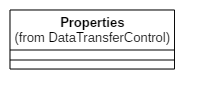
\includegraphics[width=0.25\linewidth]{images/graphite/classes/ClassProperties}
\end{figure} 
\subsubsection{Declaration}{
\begin{lstlisting}[frame=none]
public class Properties
 extends java.lang.Object\end{lstlisting}
\subsubsection{Constructor summary}{
\begin{verse}
\hyperlink{DataTransferControl.Properties()}{{\bf Properties()}} Default constructor\\
\end{verse}
}
\subsubsection{Constructors}{
\vskip -2em
\begin{itemize}
\item{ 
\index{Properties()}
\hypertarget{DataTransferControl.Properties()}{{\bf  Properties}\\}
\begin{lstlisting}[frame=none]
public Properties()\end{lstlisting} %end signature
\begin{itemize}
\item{
{\bf  Description}

Default constructor
}
\end{itemize}
}%end item
\end{itemize}
}
}
\subsection{\label{DataTransferControl.Sender}Class Sender}{
\hypertarget{DataTransferControl.Sender}{}\vskip .1in 
Reformats the data and sends it to another component\vskip .1in 
\begin{figure}[!htp]
	\centering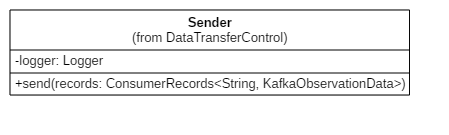
\includegraphics[width=0.6\linewidth]{images/graphite/classes/ClassSender}
\end{figure} 
\subsubsection{Declaration}{
\begin{lstlisting}[frame=none]
public class Sender
 extends java.lang.Object\end{lstlisting}
\subsubsection{All known subclasses}{GraphiteSender\small{\refdefined{DataTransferControl.GraphiteSender}}}
\subsubsection{Constructor summary}{
\begin{verse}
\hyperlink{DataTransferControl.Sender()}{{\bf Sender()}} Default constructor\\
\end{verse}
}
\subsubsection{Method summary}{
\begin{verse}
\hyperlink{DataTransferControl.Sender.send(<any>)}{{\bf send()}} Sends the resulting data to the specified component\\
\end{verse}
}
\subsubsection{Constructors}{
\vskip -2em
\begin{itemize}
\item{ 
\index{Sender()}
\hypertarget{DataTransferControl.Sender()}{{\bf  Sender}\\}
\begin{lstlisting}[frame=none]
public Sender()\end{lstlisting} %end signature
\begin{itemize}
\item{
{\bf  Description}

Default constructor
}
\end{itemize}
}%end item
\end{itemize}
}
\subsubsection{Methods}{
\vskip -2em
\begin{itemize}
\item{ 
\index{send()}
\hypertarget{DataTransferControl.Sender.send(<any>)}{{\bf  send}\\}
\begin{lstlisting}[frame=none]
public void send(ConsumerRecords<String, KafkaObservationData> records)\end{lstlisting} %end signature
\begin{itemize}
\item{
{\bf  Description}

Sends the resulting data to the specified component
}
\item{
{\bf  Parameters}
  \begin{itemize}
   \item{
\texttt{records} -- Multiple records of data from Kafka}
  \end{itemize}
}%end item
\end{itemize}
}%end item
\end{itemize}
}
}
\subsection{\label{DataTransferControl.Servet}Class Servlet}{
\hypertarget{DataTransferControl.Servet}{}\vskip .1in 
A Servlet, which accepts the user-requests from the webinterface and passes them on to the responsible structures\vskip .1in
\begin{figure}[!htp]
	\centering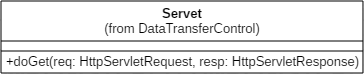
\includegraphics[width=0.5\linewidth]{images/graphite/classes/ClassServlet}
\end{figure} 
\subsubsection{Declaration}{
\begin{lstlisting}[frame=none]
public class Servet
 extends java.lang.Object\end{lstlisting}
\subsubsection{Constructor summary}{
\begin{verse}
\hyperlink{DataTransferControl.Servet()}{{\bf Servet()}} Default constructor\\
\end{verse}
}
\subsubsection{Method summary}{
\begin{verse}
\hyperlink{DataTransferControl.Servet.doGet(HttpServletRequest, HttpServletResponse)}{{\bf doGet(HttpServletRequest, HttpServletResponse)}} Receives the information of the data, that will be send back\\
\end{verse}
}
\subsubsection{Constructors}{
\vskip -2em
\begin{itemize}
\item{ 
\index{Servet()}
\hypertarget{DataTransferControl.Servet()}{{\bf  Servet}\\}
\begin{lstlisting}[frame=none]
public Servet()\end{lstlisting} %end signature
\begin{itemize}
\item{
{\bf  Description}

Default constructor
}
\end{itemize}
}%end item
\end{itemize}
}
\subsubsection{Methods}{
\vskip -2em
\begin{itemize}
\item{ 
\index{doGet(HttpServletRequest, HttpServletResponse)}
\hypertarget{DataTransferControl.Servet.doGet(HttpServletRequest, HttpServletResponse)}{{\bf  doGet}\\}
\begin{lstlisting}[frame=none]
public void doGet(HttpServletRequest req,HttpServletResponse resp)\end{lstlisting} %end signature
\begin{itemize}
\item{
{\bf  Description}

Receives the information of the data, that will be send back
}
\item{
{\bf  Parameters}
  \begin{itemize}
   \item{
\texttt{req} -- A http servlet request}
   \item{
\texttt{resp} -- A http servlet response}
  \end{itemize}
}%end item
\end{itemize}
}%end item
\end{itemize}
}
}
}
\section{Package DataTransferControl.SerializationDeserialization}{
\label{DataTransferControl.SerializationDeserialization}\hypertarget{DataTransferControl.SerializationDeserialization}{}
\hskip -.05in
\hbox to \hsize{\textit{ Package Contents\hfil Page}}
\vskip .13in
\hbox{{\bf  Classes}}
\entityintro{KafkaObservationData}{DataTransferControl.SerializationDeserialization.KafkaObservationData}{A serializable object that contains the observed data from kafka}
\entityintro{ObservationDataDeserializer}{DataTransferControl.SerializationDeserialization.ObservationDataDeserializer}{Deserializes KafkaObservationData objects}
\vskip .1in
\vskip .1in
\subsection{\label{DataTransferControl.SerializationDeserialization.KafkaObservationData}Class KafkaObservationData}{
\hypertarget{DataTransferControl.SerializationDeserialization.KafkaObservationData}{}\vskip .1in 
A serializable object that contains the observed data from kafka\vskip .1in 
\begin{figure}[!htp]
	\centering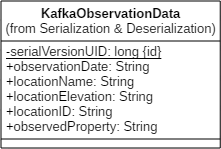
\includegraphics[width=0.3\linewidth]{images/graphite/classes/ClassKafkaObservationData}
\end{figure} 
\subsubsection{Declaration}{
\begin{lstlisting}[frame=none]
public class KafkaObservationData
 extends java.lang.Object implements java.io.Serializable\end{lstlisting}
\subsubsection{Field summary}{
\begin{verse}
\hyperlink{DataTransferControl.SerializationDeserialization.KafkaObservationData.locationElevation}{{\bf locationElevation}} The height of the observations location\\
\hyperlink{DataTransferControl.SerializationDeserialization.KafkaObservationData.locationID}{{\bf locationID}} The id of the observations location\\
\hyperlink{DataTransferControl.SerializationDeserialization.KafkaObservationData.locationName}{{\bf locationName}} The name of the observations location\\
\hyperlink{DataTransferControl.SerializationDeserialization.KafkaObservationData.observationDate}{{\bf observationDate}} The date of the observation\\
\hyperlink{DataTransferControl.SerializationDeserialization.KafkaObservationData.observedProperty}{{\bf observedProperty}} The observed property\\
\end{verse}
}
\subsubsection{Constructor summary}{
\begin{verse}
\hyperlink{DataTransferControl.SerializationDeserialization.KafkaObservationData()}{{\bf KafkaObservationData()}} Default constructor\\
\end{verse}
}
\subsubsection{Fields}{
\begin{itemize}
\item{
\index{observationDate}
\label{DataTransferControl.SerializationDeserialization.KafkaObservationData.observationDate}\hypertarget{DataTransferControl.SerializationDeserialization.KafkaObservationData.observationDate}{\texttt{public java.lang.String\ {\bf  observationDate}}
}
\begin{itemize}
\item{\vskip -.9ex 
The date of the observation}
\end{itemize}
}
\item{
\index{locationName}
\label{DataTransferControl.SerializationDeserialization.KafkaObservationData.locationName}\hypertarget{DataTransferControl.SerializationDeserialization.KafkaObservationData.locationName}{\texttt{public java.lang.String\ {\bf  locationName}}
}
\begin{itemize}
\item{\vskip -.9ex 
The name of the observations location}
\end{itemize}
}
\item{
\index{locationElevation}
\label{DataTransferControl.SerializationDeserialization.KafkaObservationData.locationElevation}\hypertarget{DataTransferControl.SerializationDeserialization.KafkaObservationData.locationElevation}{\texttt{public java.lang.String\ {\bf  locationElevation}}
}
\begin{itemize}
\item{\vskip -.9ex 
The height of the observations location}
\end{itemize}
}
\item{
\index{locationID}
\label{DataTransferControl.SerializationDeserialization.KafkaObservationData.locationID}\hypertarget{DataTransferControl.SerializationDeserialization.KafkaObservationData.locationID}{\texttt{public java.lang.String\ {\bf  locationID}}
}
\begin{itemize}
\item{\vskip -.9ex 
The id of the observations location}
\end{itemize}
}
\item{
\index{observedProperty}
\label{DataTransferControl.SerializationDeserialization.KafkaObservationData.observedProperty}\hypertarget{DataTransferControl.SerializationDeserialization.KafkaObservationData.observedProperty}{\texttt{public java.lang.String\ {\bf  observedProperty}}
}
\begin{itemize}
\item{\vskip -.9ex 
The observed property}
\end{itemize}
}
\end{itemize}
}
\subsubsection{Constructors}{
\vskip -2em
\begin{itemize}
\item{ 
\index{KafkaObservationData()}
\hypertarget{DataTransferControl.SerializationDeserialization.KafkaObservationData()}{{\bf  KafkaObservationData}\\}
\begin{lstlisting}[frame=none]
public KafkaObservationData()\end{lstlisting} %end signature
\begin{itemize}
\item{
{\bf  Description}

Default constructor
}
\end{itemize}
}%end item
\end{itemize}
}
}
\subsection{\label{DataTransferControl.SerializationDeserialization.ObservationDataDeserializer}Class ObservationDataDeserializer}{
\hypertarget{DataTransferControl.SerializationDeserialization.ObservationDataDeserializer}{}\vskip .1in 
Deserializes KafkaObservationData objects\vskip .1in 
\begin{figure}[!htp]
	\centering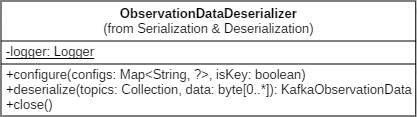
\includegraphics[width=0.65\linewidth]{images/graphite/classes/ClassObservationDataDeserializer}
\end{figure} 
\subsubsection{Declaration}{
\begin{lstlisting}[frame=none]
public class ObservationDataDeserializer
 extends java.lang.Object\end{lstlisting}
\subsubsection{Constructor summary}{
\begin{verse}
\hyperlink{DataTransferControl.SerializationDeserialization.ObservationDataDeserializer()}{{\bf ObservationDataDeserializer()}} Default constructor\\
\end{verse}
}
\subsubsection{Method summary}{
\begin{verse}
\hyperlink{DataTransferControl.SerializationDeserialization.ObservationDataDeserializer.close()}{{\bf close()}} Closes this object\\
\hyperlink{DataTransferControl.SerializationDeserialization.ObservationDataDeserializer.configure(java.util.Map, boolean)}{{\bf configure(Map, boolean)}} Configures the deserializer\\
\hyperlink{DataTransferControl.SerializationDeserialization.ObservationDataDeserializer.deserialize(java.util.Collection, java.util.Set)}{{\bf deserialize(Collection, Set)}} Deserializes an object\\
\end{verse}
}
\subsubsection{Constructors}{
\vskip -2em
\begin{itemize}
\item{ 
\index{ObservationDataDeserializer()}
\hypertarget{DataTransferControl.SerializationDeserialization.ObservationDataDeserializer()}{{\bf  ObservationDataDeserializer}\\}
\begin{lstlisting}[frame=none]
public ObservationDataDeserializer()\end{lstlisting} %end signature
\begin{itemize}
\item{
{\bf  Description}

Default constructor
}
\end{itemize}
}%end item
\end{itemize}
}
\subsubsection{Methods}{
\vskip -2em
\begin{itemize}
\item{ 
\index{close()}
\hypertarget{DataTransferControl.SerializationDeserialization.ObservationDataDeserializer.close()}{{\bf  close}\\}
\begin{lstlisting}[frame=none]
public void close()\end{lstlisting} %end signature
\begin{itemize}
\item{
{\bf  Description}

Closes this object
}
\end{itemize}
}%end item
\item{ 
\index{configure(Map, boolean)}
\hypertarget{DataTransferControl.SerializationDeserialization.ObservationDataDeserializer.configure(java.util.Map, boolean)}{{\bf  configure}\\}
\begin{lstlisting}[frame=none]
public void configure(java.util.Map configs,boolean isKey)\end{lstlisting} %end signature
\begin{itemize}
\item{
{\bf  Description}

Configures the deserializer
}
\item{
{\bf  Parameters}
  \begin{itemize}
   \item{
\texttt{configs} -- The Configuration}
   \item{
\texttt{isKey} -- A variable, telling us whether we want to configure the key or the value}
  \end{itemize}
}%end item
\end{itemize}
}%end item
\item{ 
\index{deserialize(Collection, Set)}
\hypertarget{DataTransferControl.SerializationDeserialization.ObservationDataDeserializer.deserialize(java.util.Collection, java.util.Set)}{{\bf  deserialize}\\}
\begin{lstlisting}[frame=none]
public KafkaObservationData deserialize(java.util.Collection topics,java.util.Set data)\end{lstlisting} %end signature
\begin{itemize}
\item{
{\bf  Description}

Deserializes an object
}
\item{
{\bf  Parameters}
  \begin{itemize}
   \item{
\texttt{topics} -- Kafka-Topics that should be subscribed}
   \item{
\texttt{data} -- These are our serialized bytes}
  \end{itemize}
}%end item
\item{{\bf  Returns} -- 
A serializable object that contains the observed data from kafka 
}%end item
\end{itemize}
}%end item
\end{itemize}
}
}
}
